\documentclass[a4paper,12pt]{book}

\usepackage[english]{babel}
\usepackage{blindtext}
\usepackage{microtype}
\usepackage{graphicx}
\usepackage{wrapfig}
\usepackage{enumitem}
\usepackage{fancyhdr}
\usepackage{amsmath}
\usepackage{index}

\makeindex

\begin{document}
\title{\Large{\textbf{LaTeX Tutorial}}}
\author{By Humphrey Curtis}
\date{12 April 2020}

\maketitle 
\let\cleardoublepage\clearpage
\tableofcontents 

\pagenumbering{roman}
\setcounter{page}{2}

\chapter{Chapter Name}

\blindmathtrue
\blindtext[5]

\section{A Section}
\blindtext
\begin{figure}[ht]
\centering 

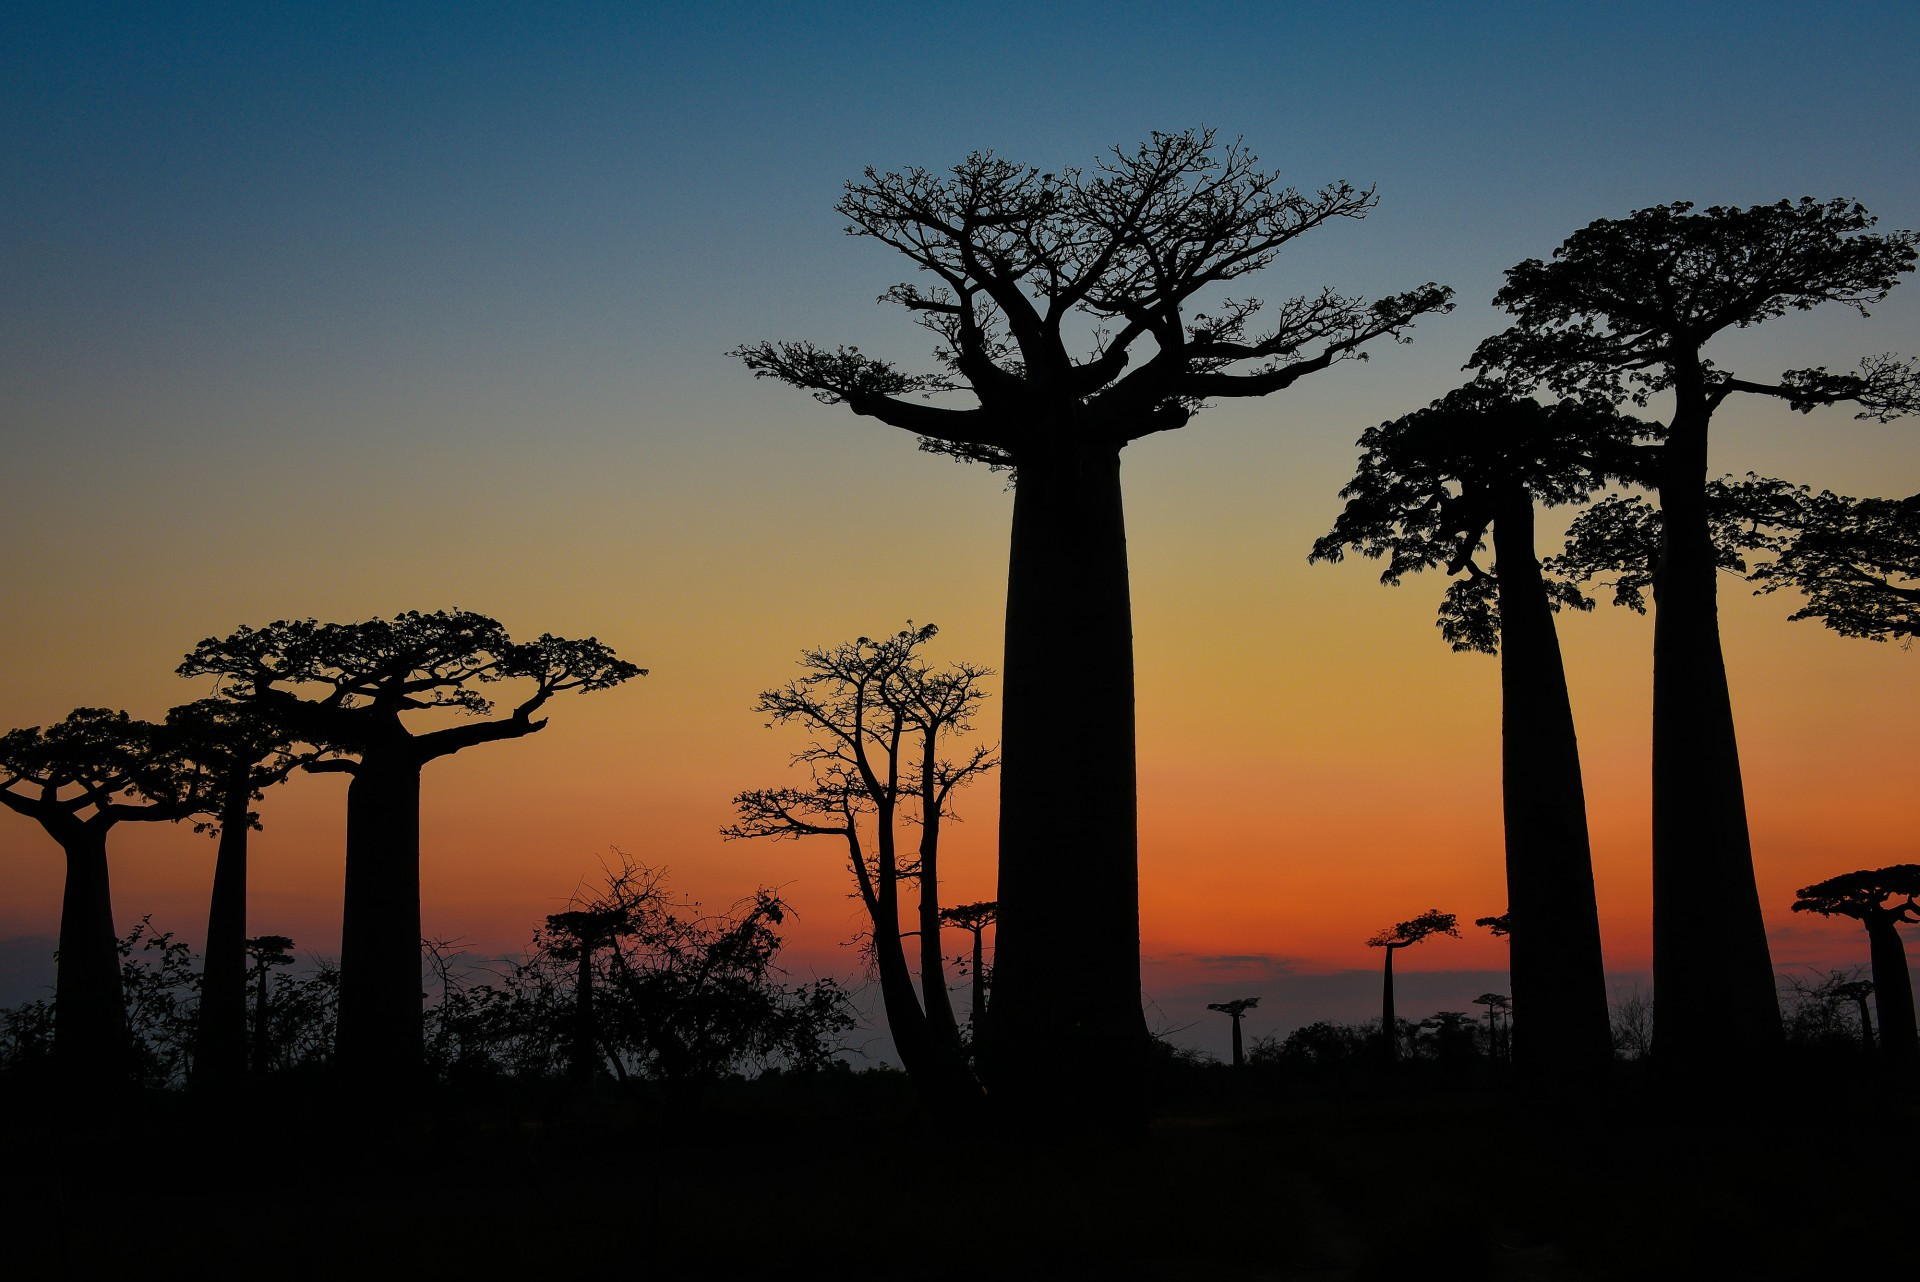
\includegraphics[width=8cm]{pic.png}
\end{figure}
\blindtext
\newpage

\section*{Wrap Image}
\begingroup
\setlength{\intextsep}{0pt}
\setlength{\columnsep}{15pt}

\begin{wrapfigure}{r}{0.45\textwidth}
\centering
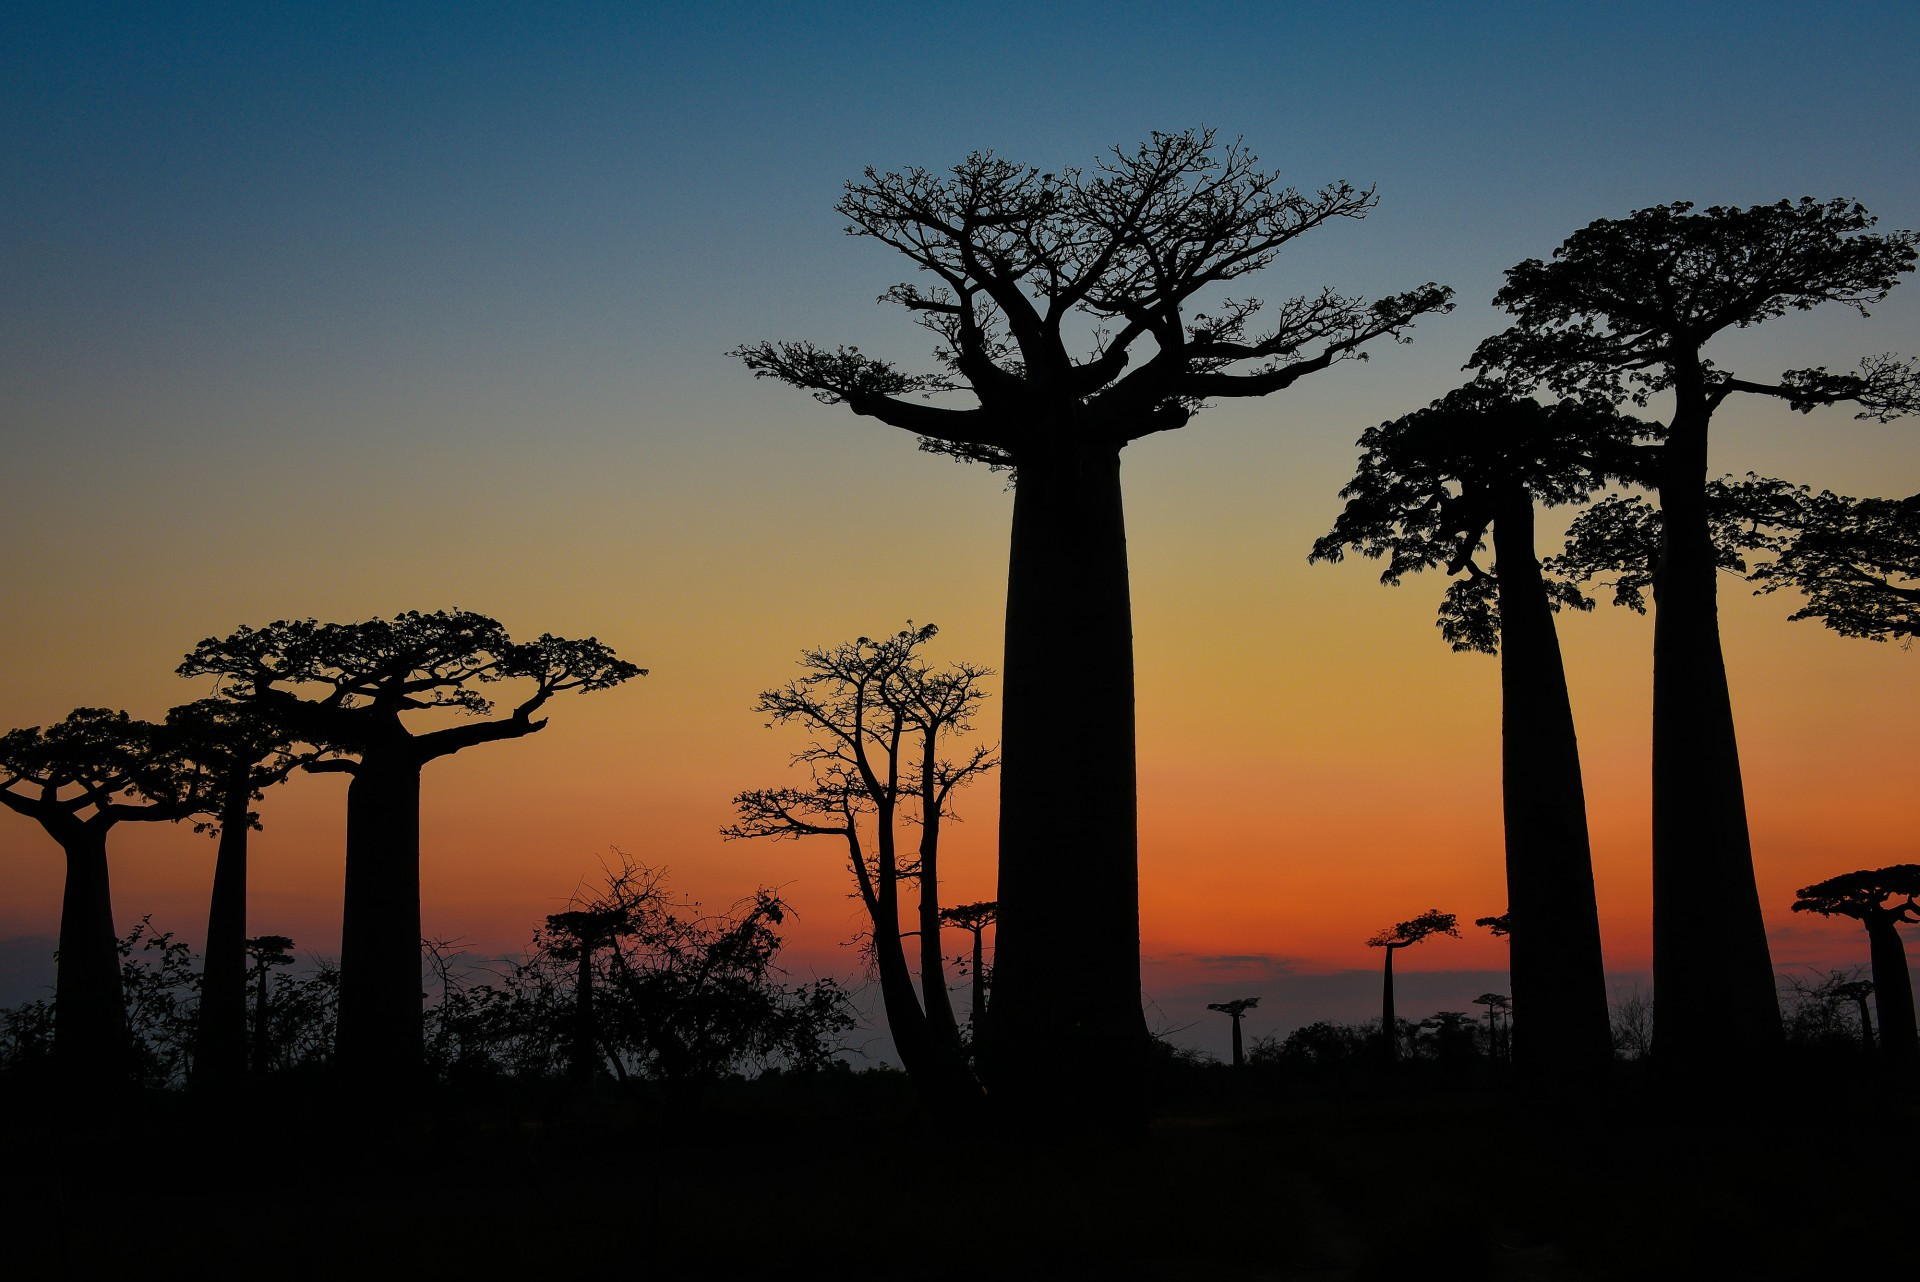
\includegraphics[width=\linewidth]{pic.png}
\caption{Pretty picture}\label{fig:prettypic}
\end{wrapfigure}

\blindtext

\endgroup

\section{Smoothie Recipe}
\begin{itemize}
	\item 1 Cup Spinach
	\item 1 Cup Frozen Blueberries 
	\item 2 Bananas 
\end{itemize}


\section{Smoothie}
\blindtext[2]

\section{Perfect Meal Recipe}
\blindtext[2]

\end{document}